\chapter{FEM}

\section{General Statements}
The simulation domain is seen in Fig.
%---------------------------------------------------------------------------------------------------------------
\begin{figure}[H]
	\centering
	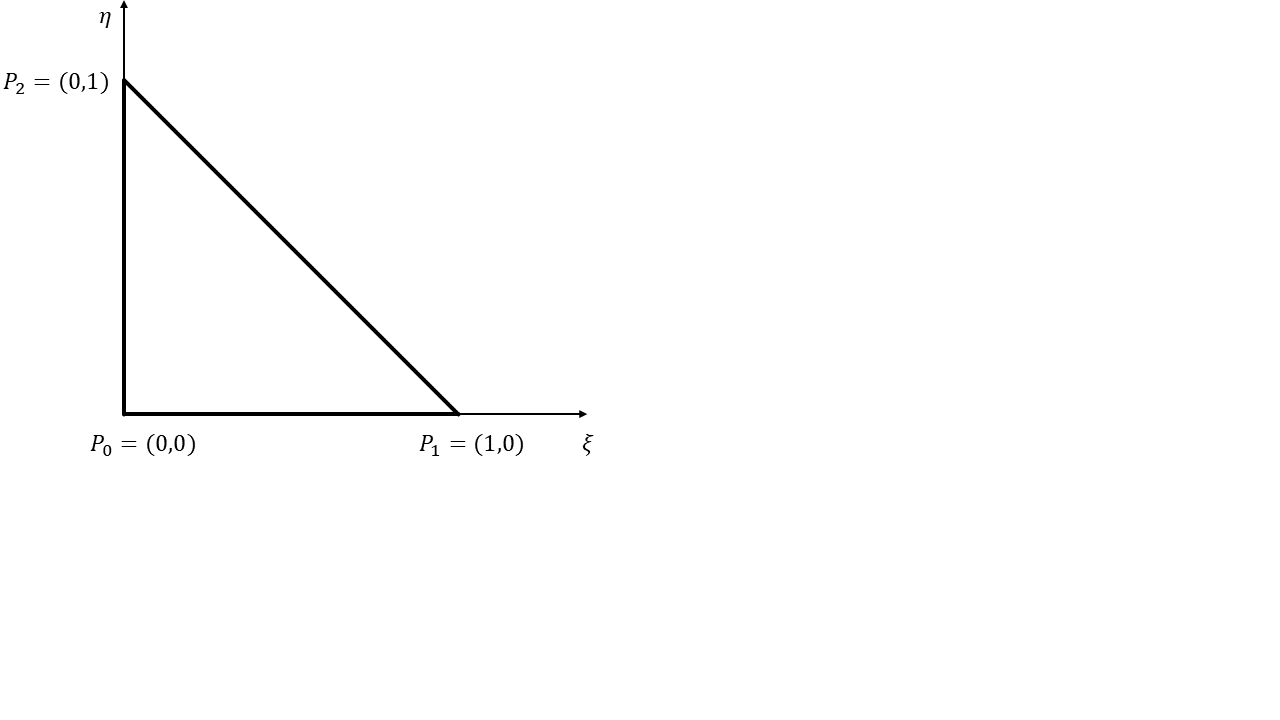
\includegraphics[trim= 0cm 7cm 18cm 0cm ,clip,width=0.6\textwidth]{figures/FEM_triangle.png}
	\caption{Radiation.}
	\label{fig:FEM_domain}
\end{figure}
%---------------------------------------------------------------------------------------------------------------
Using the definitions
\begin{align}
	x_i &\equiv P_{i,x} \\
	y_i &\equiv P_{i,y}
\end{align}
and
\begin{align}
	\Delta x_k &= x_0 - x_k\\
	\Delta y_k &= y_0 - y_k
\end{align}
the cartesian coordinates can be expressed in terms of the new coordinates as
\begin{align}
	x(\xi, \eta) &= x_0 + \Delta x_1 \xi + \Delta x_2 \eta\\
	y(\xi, \eta) &= y_0 + \Delta y_1 \xi + \Delta y_2 \eta
\end{align}
and the new coordinates as
\begin{align}
	\xi(x, y) & = \frac{1}{\det\left(\mm{J}(x,y) \right)} \big(\Delta y_2 (x - x_0) - \Delta x_2 (y - y_0) \big)\\
	\eta(x, y) & = \frac{1}{\det\left(\mm{J}(x,y) \right)} \big(-\Delta y_1 (x - x_0) + \Delta x_1(y - y_0) \big)
\end{align}
with the Jacobian matrix
\begin{equation}
	\mm{J}(x,y) =
	\begin{bmatrix}
	x_{\xi} & x_{\eta} \\
	y_{\xi} & y_{\eta}
	\end{bmatrix}
	=
	\begin{bmatrix}
	\Delta x_{1} & \Delta x_{2}\\
	\Delta y_{1} & \Delta y_{2}
	\end{bmatrix}
\end{equation}
and its determinant
\begin{equation}
	\det\left(\mm{J}(x, y)\right) = \Delta x_1 \Delta y_2 - \Delta x_2 \Delta y_1.
\end{equation}
The Jacobian for the backward transformation can be expressed as
\begin{equation}
	\mm{J}(\xi, \eta) = 
	\begin{bmatrix}
	\xi_{x} & \xi_{y} \\
	\eta_{x} & \eta_{y}
	\end{bmatrix}
	= \frac{1}{\det\left(\mm{J}(x,y)\right)}
	\begin{bmatrix}
	\Delta y_{2} & -\Delta x_{2}\\
	-\Delta y_{1} & \Delta x_{1}
	\end{bmatrix}
\end{equation}
and its determinant
\begin{equation}
	\det\left( \mm{J}(\xi, \eta) \right) = \frac{\Delta x_1 \Delta y_2 + \Delta x_2 \Delta y_1}{\Delta x_1 \Delta y_2 - \Delta x_2 \Delta y_1}.
\end{equation}
Required derivatives can be transformed as
\begin{align}
	\pdv{u(\xi, \eta)}{x} &= \pdv{u}{\xi}\pdv{\xi}{x} + \pdv{u}{\eta}\pdv{\eta}{x}\\
	\pdv{u(\xi, \eta)}{y} &= \pdv{u}{\xi}\pdv{\xi}{y} + \pdv{u}{\eta}\pdv{\eta}{y}.
\end{align}
With use tetrahedral ansatz functions $\phi(\xi, \eta)$ with the definition
\begin{equation}
	\phi_i \equiv \phi(P_i)
\end{equation}
which can be explicitly given as for the new coordinate system as
\begin{align}
	\phi_0(\xi, \eta) &= -\xi - \eta  + 1\\
	\phi_1(\xi, \eta) &= \xi\\
	\phi_2(\xi, \eta) &= \eta.
\end{align}
Using this ansatz function the temperature is defined in the support space as
\begin{equation}
	T(\xi, \theta)  = \sum_i^3 T_i \phi_i
\end{equation}
and its gradient
\begin{align}
	\nabla T(\xi, \eta) &=
	\begin{pmatrix}
	\pdv{T}{\xi}\pdv{\xi}{x} + \pdv{T}{\eta}\pdv{\eta}{x}\\
	\pdv{T}{\xi}\pdv{\xi}{y} + \pdv{T}{\eta}\pdv{\eta}{y}
	\end{pmatrix}\\
	&= \frac{1}{\det\left(\mm{J}(x,y)\right)}
	\begin{pmatrix}
	(-T_0 + T_1)\Delta y_2 - (-T_0 + T_2)\Delta y_1\\
	-(-T_0 + T_1)\Delta x_2 + (-T_0 + T_2)\Delta x_1
	\end{pmatrix}\\
	&= \frac{1}{\det\left(\mm{J}(x,y)\right)}
	\begin{pmatrix}
	T_0(\Delta y_1 - \Delta y_2) + T_1\Delta y_2 - T_2\Delta y_1\\
	T_0(\Delta x_2 - \Delta x_1) - T_1 \Delta x_2 + T_2 \Delta x_1
	\end{pmatrix}.
\end{align}
